%!TEX root = /Users/louis/Documents/PhD/Deliverables/Thesis/thesis.tex

\chapter[A Graphical Editor for Process-Oriented Programs][An Exemplar Graphical Model Editor]{A Graphical Editor for Process-Oriented Programs}
\label{ProcessOriented}

The way in which a prototypical graphical editor for process-oriented programs was designed and implemented is described in this appendix. The work presented here was conducted in collaboration with Adam Sampson, then a Research Associate at the University of Kent. The way in which the graphical editor changed throughout its development provided was used for evaluation of the thesis research in Section~\ref{sec:exemplar_user-driven_co-evo}.

The purpose of the collaboration was to explore the suitability of MDE tools and techniques for designing a graphical notation and supporting tools for programs written in process-oriented programming languages, such as occam-$\pi$ \cite{occam_pi}. The collaboration resulted in the design and implementation of a prototypical graphical editor, which was used to construct examples of small process-oriented programs.

Process-oriented programs are specified in terms of three core concepts: processes, connection points and channels. Processes are the fundamental building blocks of a process-oriented program. Channels are the mechanism by which processes communicate, and are unidirectional. Connection points define the channels on which a process can communicate. Connection points are used to specify the way in which a process can communicate, and can optionally be bound to a channel. Because channels are unidirectional, connection points are either reading (consume messages from the channel) or writing (generate messages on the channel).

MDE tools and techniques were used to design and implement a graphical notation and editor for process-oriented programs by Sampson and the thesis author. An iterative style of development was used. The abstract syntax of the domain was specified as a metamodel, captured in Ecore, which is the metamodelling language of arguably the most widely-used contemporary MDE development environment, the Eclipse Modeling Framework (EMF) \cite{steinberg09emf}. The graphical concrete syntax was specified with the Graphical Modeling Framework (GMF) \cite{gronback06gmf}, via EuGENia, \cite{kolovos09eugenia}. EMF and GMF are described more thoroughly in Section~\ref{sec:mde_tools}.

The remainder of this appendix presents the six versions of the process-oriented metamodel constructed by Sampson and the thesis author during the iterative development of the graphical editor. In addition, several models are also shown, which were used to test the graphical editor throughout its development. 

\section{Iteration 1: Processes and Channels}
Development began by identifying two key concepts for modelling process-oriented programs. From examples of process-oriented programs, process and channel were identified as the most important concepts, and consequently the metamodel shown in Figure~\ref{fig:po_it1_mm} was constructed.


\begin{figure}[htbp]
	\centering
		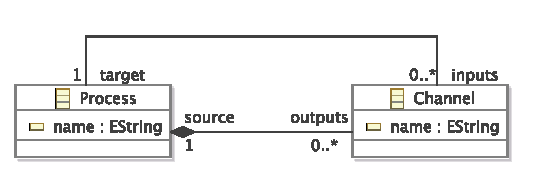
\includegraphics[scale=0.75]{A.2.ProcessOriented/images/1_mm.pdf}
	\caption{The process-oriented metamodel after the first iteration.}
	\label{fig:po_it1_mm}
\end{figure}

Additionally, a graphical concrete syntax was chosen for processes and channels. The former were represented as boxes, and the latter as lines. EuGENia annotations were added to the metamodel, resulting in the metamodel shown in Listing~\ref{lst:po_it1_mm}. Line 1 of Listing~\ref{lst:po_it1_mm} uses the ``@gmf.node'' EuGENia annotation to indicate that processes are to be represented as boxes with a label equal to the value of the \texttt{name} feature. Line 9 uses the ``@gmf.link'' EuGENia annotation to indicate that channels are to be represented as lines between \texttt{source} and \texttt{target} processes with a label equal to the value of the \texttt{name} feature. 

\begin{lstlisting}[caption=The annotated process-oriented metamodel after the first iteration, label=lst:po_it1_mm, language=Emfatic]
@gmf.node(label="name")
class Process {
   attr String name;
      
   ref Channel[*]#target inputs;
   val Channel[*]#source outputs; 
}

@gmf.link(source="source", target="target", label="name")
class Channel { 
   attr String name;
   ref Process[1]#outputs source;
   ref Process[1]#inputs target;
} 

\end{lstlisting}

To generate code for the graphical editor, EuGENia was invoked on the annotated metamodel shown in Listing~\ref{lst:po_it1_mm}. However, EuGENia failed with an error, because no ``root'' element had been specified. GMF, the graphical modelling framework used by EuGENia, requires one metaclass (termed the root) to be specified as a container for all diagram elements. The root metaclass cannot be a GMF node or a link, and so the second iteration involved adding an additional metaclass for interoperability with GMF.


\section{Iteration 2: Interoperability with GMF}
In the second iteration, an additional metaclass, \texttt{Model}, was added to the metamodel as shown in Figure~\ref{fig:po_it2_mm}. The \texttt{Model} metaclass was used to provide GMF with a container for storing all of the diagram elements for each process-oriented diagram.

\begin{figure}[htbp]
	\centering
		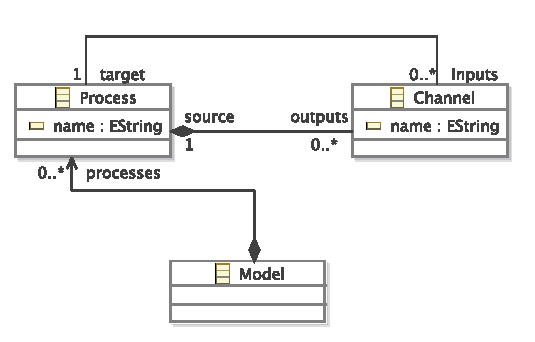
\includegraphics[scale=0.75]{A.2.ProcessOriented/images/2_mm.pdf}
	\caption{The process-oriented metamodel after the second iteration.}
	\label{fig:po_it2_mm}
\end{figure}

As shown in Listing~\ref{lst:po_it1_mm}, the \texttt{Model} metaclass was annotated with ``@gmf.diagram'' to indicate that it should be used as the diagram's root element. Root elements do not have a concrete syntax and do not appear in the graphical editor.

\begin{lstlisting}[caption=The annotated process-oriented metamodel after the second iteration, label=lst:po_it2_mm, language=Emfatic]
@gmf.diagram
class Model {
   val Process[*] processes;
}

@gmf.node(label="name")
class Process {
   attr String name;
      
   ref Channel[*]#target inputs;
   val Channel[*]#source outputs; 
}


@gmf.link(source="source", target="target", label="name")
class Channel { 
   attr String name;
   ref Process[1]#outputs source;
   ref Process[1]#inputs target;
}
\end{lstlisting}

EuGENia was invoked on the annotated metamodel shown in Listing~\ref{lst:po_it2_mm} to produce code for the graphical editor. Figure~\ref{fig:po_it2_model} shows a simplistic test model, which was constructed to test the generated editor. The model shown in Figure~\ref{fig:po_it2_model} comprises two processes, \texttt{P1} and \texttt{P2}, and one channel, \texttt{a}.

\begin{figure}[htbp]
	\centering
		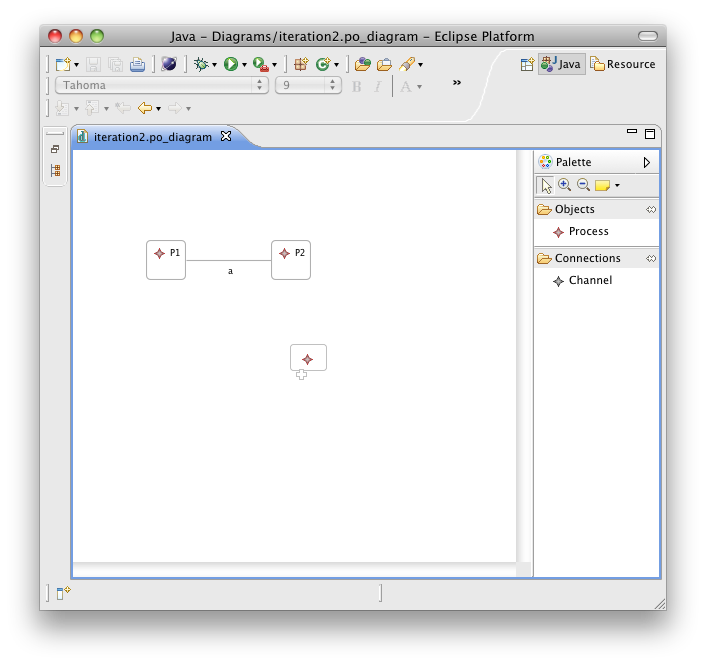
\includegraphics[scale=0.5]{A.2.ProcessOriented/images/2_model.png}
	\caption{Exemplar diagram after the second iteration.}
	\label{fig:po_it2_model}
\end{figure}

\section{Iteration 3: Shared Channels}
In previous iterations, channels had been contained within their source process. The nested structure made it more difficult to explore process-oriented models in EMF's tree editor due to the additional level of nesting. Consequently, the metamodel was changed such that channels were contained in the root element, rather than in the source process, resulting in the metamodel shown in Figure~\ref{fig:po_it3_mm}.

\begin{figure}[htbp]
	\centering
		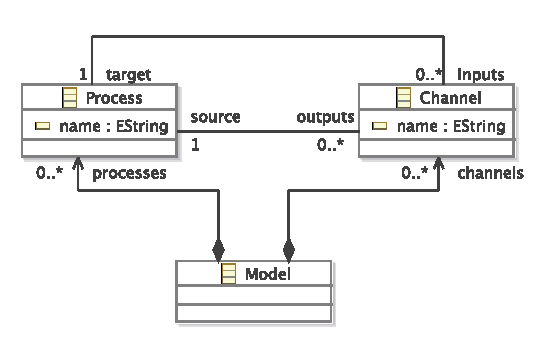
\includegraphics[scale=0.75]{A.2.ProcessOriented/images/3_mm.pdf}
	\caption{The process-oriented metamodel after the third iteration.}
	\label{fig:po_it3_mm}
\end{figure}

No additional EuGENia annotations were added to the metamodel during this iteration. In other words, the graphical notation (concrete syntax) was not changed, and the resulting editor was identical in appearance to the previous one. However, the EMF tree editor showed just one level of nesting (everything is contained inside model).

The existing models required migration because of the way in which XMI differentiates between reference and containment values. Each channel was instantiated in the new \texttt{ch\-an\-ne\-ls} reference of \texttt{Mo\-d\-el}, and existing values in the \texttt{ou\-tp\-u\-ts} reference of \texttt{Co\-nn\-ec\-ti\-onPo\-in\-t} were changed to use a reference rather than a containment value. Figure~\ref{fig:po_it3_pre} shows the HUTN for a model prior to migration, and Listing~\ref{fig:po_it3_post} shows the reconciled, migrated HUTN.

\begin{figure}[htbp]
	\centering
	\subfigure[HUTN prior to migration]
	{
	    \label{fig:po_it3_pre}
	    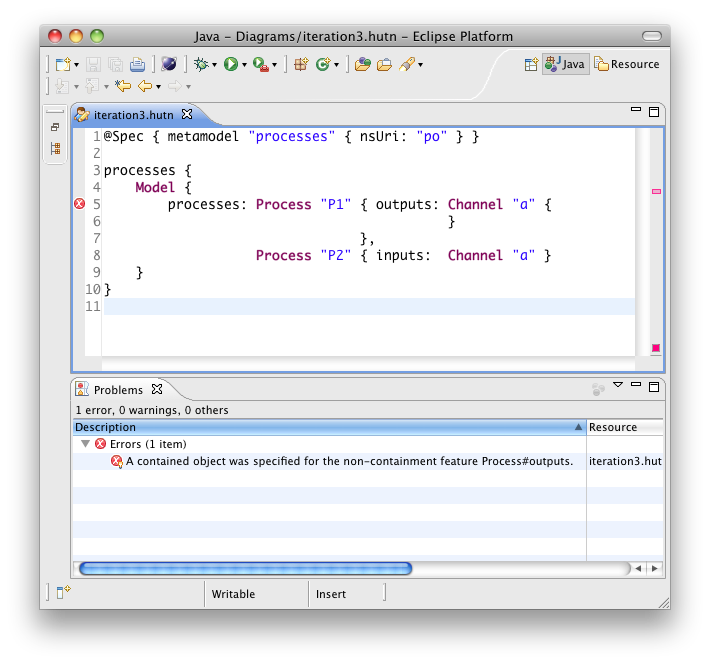
\includegraphics[width=9.5cm]{A.2.ProcessOriented/images/3_pre.png}
	}
	\subfigure[HUTN after migration]
	{
	    \label{fig:po_it3_post}
	    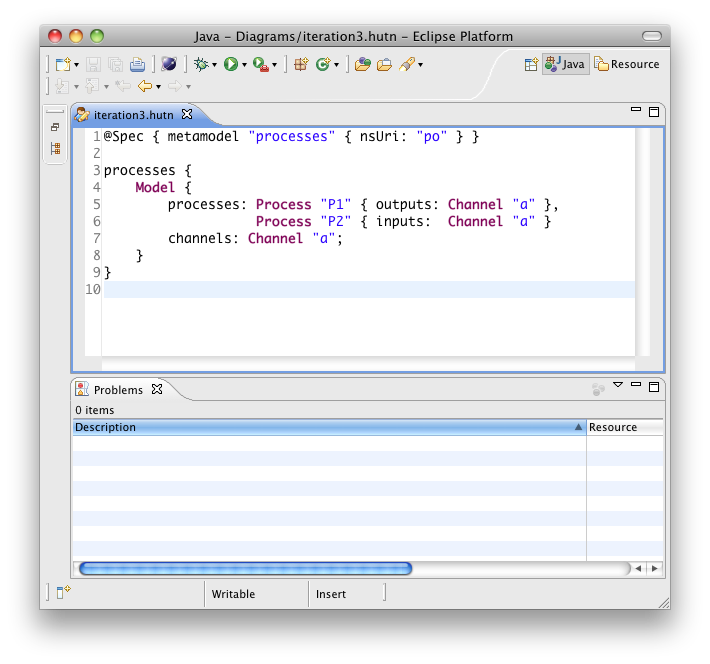
\includegraphics[width=9.5cm]{A.2.ProcessOriented/images/3_post.png}
	}
	\caption{Exemplar migration between the second and third versions of the process-oriented metamodel}
\end{figure}

\clearpage


\section{Iteration 4: Connection Points}
The fourth iteration involved capturing a third domain concept, connection points, in the graphical notation. When a process is specified, the ways in which it can communicate are declared as connection points. When a process is instantiated, channels are connected to its connection points, and messages flow in and out of the process. The graphical notation was to be used to describe both instantiated processes and types of process, the metamodel was changed to model connection points.

The iteration resulted in the metamodel shown in Figure~\ref{fig:po_it4_mm}. \texttt{Co\-nn\-ec\-ti\-o\-nP\-oi\-nt} was introduced as an association class between the \texttt{in\-pu\-ts} and \texttt{o\-ut\-pu\-ts} references.

\begin{figure}[htbp]
	\centering
		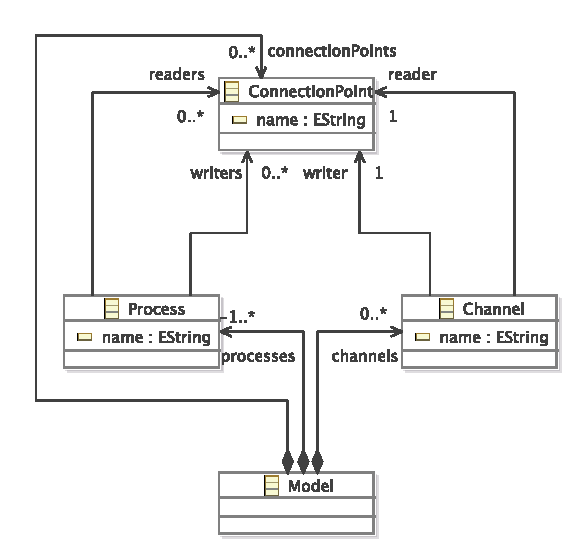
\includegraphics[scale=0.75]{A.2.ProcessOriented/images/4_mm.pdf}
	\caption{The process-oriented metamodel after the fourth iteration.}
	\label{fig:po_it4_mm}
\end{figure}

To specify concrete syntax for connection points, additional EuGENia annotations were added to the metamodel as shown in Listing~\ref{lst:po_it4mm}. The \texttt{Co\-nn\-ec\-ti\-o\-nP\-oi\-nt} class was annotated with a ``@gmf.node'' to specify that connections points were to be represented as circles, labelled with the value of the \texttt{name} attribute. The circles were to be affixed to the boxes used to represent processes, and, hence, ``@gmf.affixed'' annotations are used on lines 12 and 15.

\begin{lstlisting}[caption=The annotated process-oriented metamodel after the fourth iteration, label=lst:po_it4_mm, language=Emfatic]
@gmf.diagram
class Model {
   val Process[*] processes;
   val Channel[*] channels;
   val ConnectionPoint[*] connectionPoints;
}

@gmf.node(label="name")
class Process {
   attr String name;
      
   @gmf.affixed
   ref ConnectionPoint[*] readers;
   
   @gmf.affixed
   ref ConnectionPoint[*] writers; 
}


@gmf.link(source="reader", target="writer", label="name", incoming="true")
class Channel { 
	attr String name;
   ref ConnectionPoint[1] reader;
   ref ConnectionPoint[1] writer;
}

@gmf.node(label="name", label.placement="external", label.icon="false", figure="ellipse", size="15,15")
class ConnectionPoint {
   attr String name;
}
\end{lstlisting}

A new version of the graphical editor was generated by invoking EuGENia on the annotated metamodel. A larger test model was constructed to test the editor, and is shown in Figure~\ref{fig:po_it4_model}. The existing models required migration because the \texttt{in\-pu\-ts} and \texttt{ou\-tp\-u\-ts} references of \texttt{Pr\-oc\-e\-ss} and the \texttt{s\-ou\-r\-ce} and \texttt{ta\-rg\-et} references of \texttt{Channel} had been removed.

\begin{figure}[htbp]
	\centering
		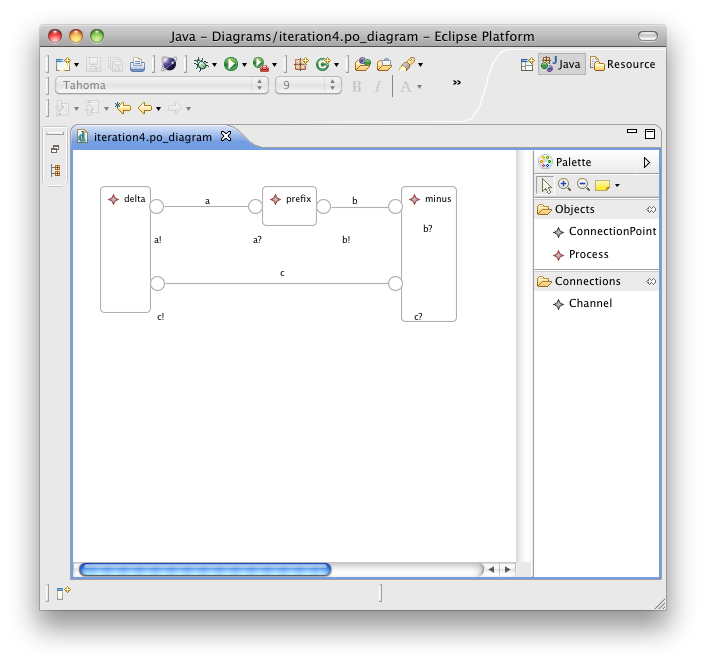
\includegraphics[scale=0.5]{A.2.ProcessOriented/images/4_model.png}
	\caption{Exemplar diagram after the fourth iteration.}
	\label{fig:po_it4_model}
\end{figure}

To migrate each existing model, two connection points were created for each channel in the model. The \texttt{s\-ou\-r\-ce} and \texttt{ta\-rg\-et} reference of the channel was changed to reference the new connection points, as were the corresponding values of the \texttt{re\-ad\-e\-rs} and \texttt{wr\-it\-e\-rs} references of the relevant processes. Figure~\ref{fig:po_it4_pre} shows the HUTN for a model prior to migration, and Figure~\ref{fig:po_it4_post} shows the reconciled, migrated HUTN.

\begin{figure}[htbp]
	\centering
	\subfigure[HUTN prior to migration]
	{
	    \label{fig:po_it4_pre}
	    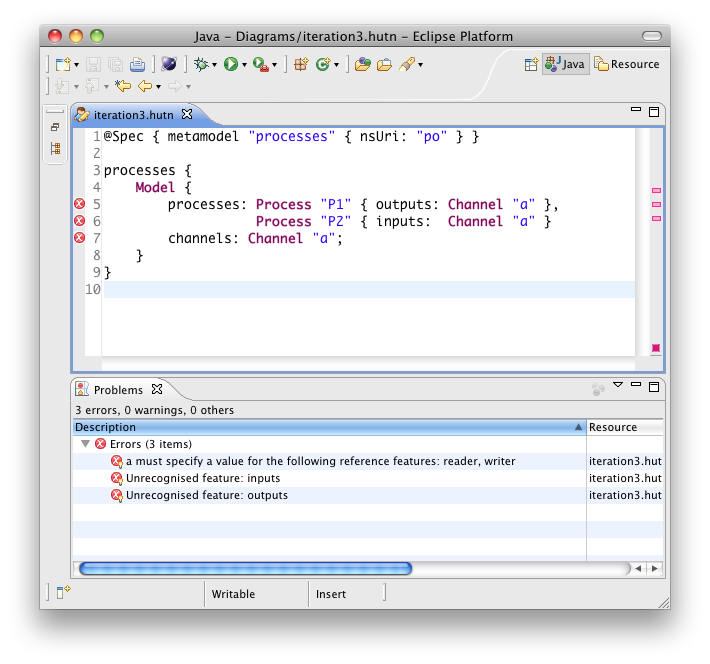
\includegraphics[width=9.5cm]{A.2.ProcessOriented/images/4_pre.png}
	}
	\subfigure[HUTN after migration]
	{
	    \label{fig:po_it4_post}
	    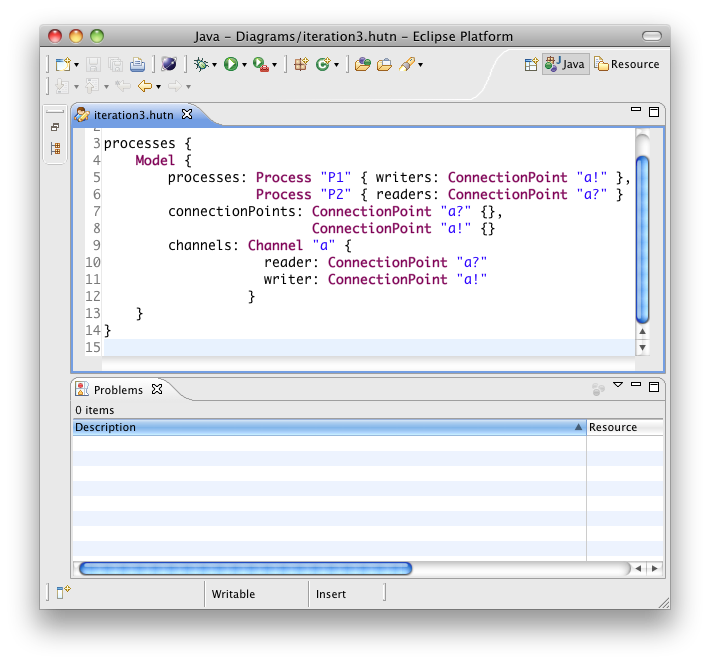
\includegraphics[width=9.5cm]{A.2.ProcessOriented/images/4_post.png}
	}
	\caption{Exemplar migration between the third and fourth versions of the process-oriented metamodel}
\end{figure}

\clearpage

\section{Iteration 5: Connection Point Types}
\label{sec:po_it5}
Channels are unidirectional, and so connection points are either \emph{reading} or \emph{writing}. A process uses the former to consume messages from a channel, and the latter to produce messages on a channel. Testing the graphical editor producing in the fourth iteration showed that it was not immediately obvious as to which connection points were reading and which were writing. The fifth iteration involved changing the graphical editor to better distinguish between reading and writing connection points.

The iteration resulted in the metamodel shown in Figure~\ref{fig:po_it5_mm}. \texttt{Co\-nn\-ec\-ti\-o\-nP\-oi\-nt} was made abstract, and two subclass, \texttt{Re\-a\-di\-ngCo\-nn\-ec\-ti\-o\-nP\-oi\-nt} and \texttt{Wr\-i\-ti\-ngCo\-nn\-ec\-ti\-o\-nP\-oi\-nt}, were introduced. The four references to \texttt{Co\-nn\-ec\-ti\-o\-nP\-oi\-nt} were changed to reference one of the two subclasses.

\begin{figure}[htbp]
	\centering
		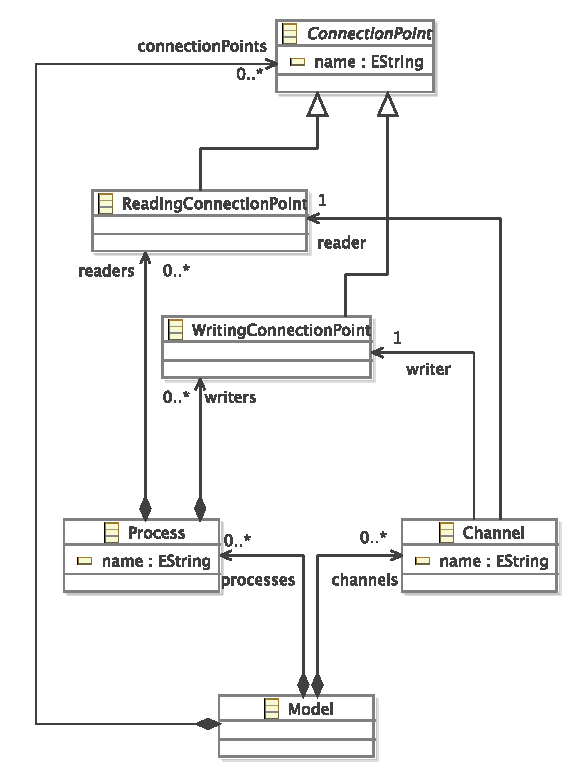
\includegraphics[scale=0.75]{A.2.ProcessOriented/images/5_mm.pdf}
	\caption{The process-oriented metamodel after the fifth iteration.}
	\label{fig:po_it5_mm}
\end{figure}

The graphical notation was changed, as shown in Listing~\ref{lst:po_it5mm}. The \texttt{Wr\-i\-ti\-ngCo\-nn\-ec\-ti\-o\-nP\-oi\-nt} class was annotated with an additional colour attribute to specify that writing connection points were to be represented with a black circle. White is the default colour for a ``@gmf.node'' annotation, and so reading connection points were represented as white circles.

\begin{lstlisting}[caption=The annotated process-oriented metamodel after the fifth iteration, label=lst:po_it5_mm, language=Emfatic]
@gmf.diagram
class Model {
   val Process[*] processes;
   val Channel[*] channels;
   val ConnectionPoint[*] connectionPoints;
}

@gmf.node(label="name")
class Process {
   attr String name;
      
   @gmf.affixed
   ref ReadingConnectionPoint[*] readers;
   
   @gmf.affixed
   ref WritingConnectionPoint[*] writers; 
}


@gmf.link(source="reader", target="writer", label="name", incoming="true")
class Channel { 
	attr String name;
   ref ReadingConnectionPoint[1] reader;
   ref WritingConnectionPoint[1] writer;
}

@gmf.node(label="name", label.placement="external", label.icon="false", figure="ellipse", size="15,15")
abstract class ConnectionPoint {
   attr String name;
}

class ReadingConnectionPoint extends ConnectionPoint {}

@gmf.node(color="0,0,0")
class WritingConnectionPoint extends ConnectionPoint {}
\end{lstlisting}

A new version of the graphical editor was generated by invoking EuGENia on the annotated metamodel. All of the existing models required migration, because \texttt{Co\-nn\-ec\-ti\-o\-nP\-oi\-nt} was now an abstract class, and could no longer be instantiated. Section~\ref{sec:exemplar_user-driven_co-evo} describes the way in which models were migrated after the changes made during this iteration. Briefly, migration involved replacing every instantiation of \texttt{Co\-nn\-ec\-ti\-o\-nP\-oi\-nt} with an instantiation of either \texttt{Re\-a\-di\-ngCo\-nn\-ec\-ti\-o\-nP\-oi\-nt} or \texttt{Wr\-i\-ti\-ngCo\-nn\-ec\-ti\-o\-nP\-oi\-nt}. The former was used when a connection point was used as the value of a channel's \texttt{re\-ad\-er} feature and the latter when  when a connection point was used as the value of a channel's \texttt{wr\-it\-er} feature. Listing~\ref{fig:po_it5_pre} shows the HUTN for a model prior to migration, and Listing~\ref{fig:po_it5_post} shows the reconciled, migrated HUTN.

\begin{figure}[htbp]
	\centering
	\subfigure[HUTN prior to migration]
	{
	    \label{fig:po_it5_pre}
	    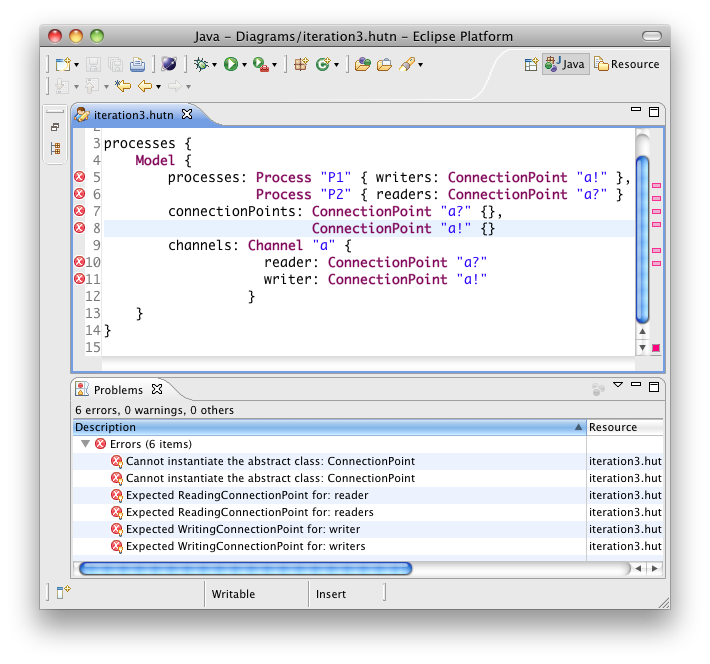
\includegraphics[width=9.5cm]{A.2.ProcessOriented/images/5_pre.png}
	}
	\subfigure[HUTN after migration]
	{
	    \label{fig:po_it5_post}
	    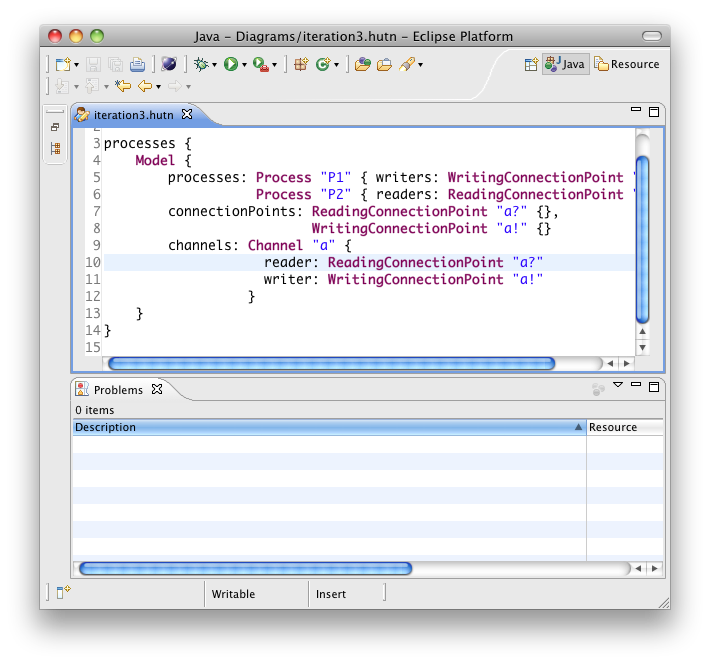
\includegraphics[width=9.5cm]{A.2.ProcessOriented/images/5_post.png}
	}
	\caption{Exemplar migration between the fourth and fifth versions of the process-oriented metamodel}
\end{figure}

\clearpage


\section{Iteration 6: Nested Processes and Channels}
The final iteration involved changing the graphical editor such that processes and channels could be nested inside other processes. In some process-oriented languages, such as occam-$\pi$ \cite{occam_pi}, processes can be specified in terms of other, internal processes.

To support the decomposition of processes into other processes and channels, the \texttt{ne\-st\-edPr\-oc\-e\-ss} and \texttt{ne\-st\-edCh\-an\-n\-el} references were added to the \texttt{Pr\-oc\-e\-ss} class, as shown in Figure~\ref{fig:po_it6_mm}. 

\begin{figure}[htbp]
	\centering
		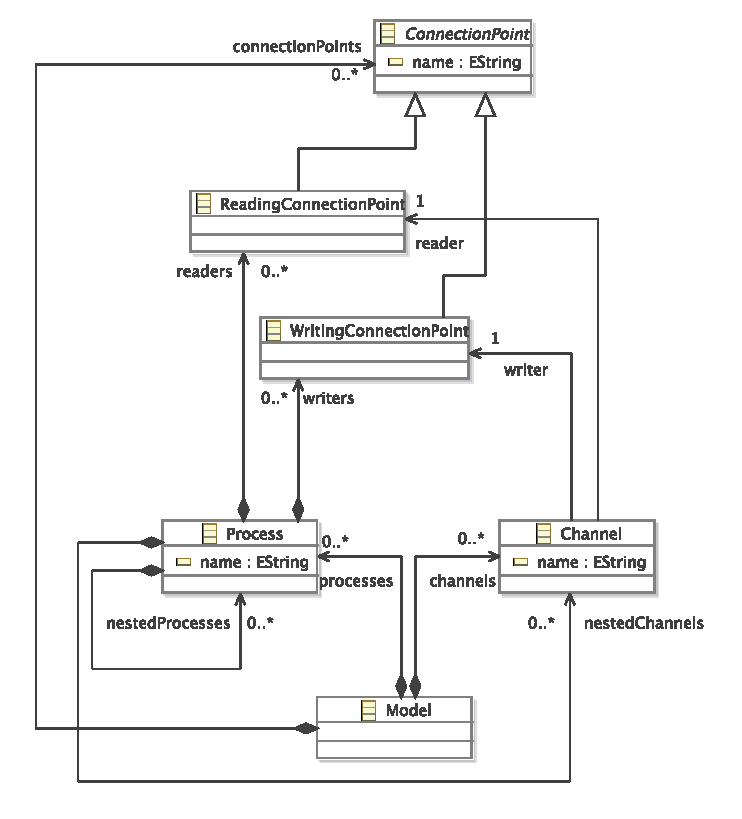
\includegraphics[scale=0.75]{A.2.ProcessOriented/images/6_mm.pdf}
	\caption{The process-oriented metamodel after the final iteration.}
	\label{fig:po_it6_mm}
\end{figure}

As shown in Listing~\ref{lst:po_it6_mm}, the ``@gmf.compartment'' annotation was added to the \texttt{ne\-st\-edPr\-oc\-e\-ss} to indicate that processes can be placed inside other processes in the graphical editor.

\begin{lstlisting}[caption=The annotated process-oriented metamodel after the final iteration, label=lst:po_it6_mm, language=Emfatic]
@gmf.diagram
class Model {
   val Process[*] processes;
   val Channel[*] channels;
   val ConnectionPoint[*] connectionPoints;
}

@gmf.node(label="name")
class Process {
   attr String name;

   @gmf.compartment
   val Process[*] nestedProcesses;
   val Channel[*] nestedChannels;
      
   @gmf.affixed
   ref ReadingConnectionPoint[*] readers;
   
   @gmf.affixed
   ref WritingConnectionPoint[*] writers; 
}


@gmf.link(source="reader", target="writer", label="name", incoming="true")
class Channel { 
	attr String name;
   ref ReadingConnectionPoint[1] reader;
   ref WritingConnectionPoint[1] writer;
}

@gmf.node(label="name", label.placement="external", label.icon="false", figure="ellipse", size="15,15")
abstract class ConnectionPoint {
   attr String name;
}

class ReadingConnectionPoint extends ConnectionPoint {}

@gmf.node(color="0,0,0")
class WritingConnectionPoint extends ConnectionPoint {}
\end{lstlisting}

EuGENia was invoked on the annotated metamodel to produce the final version of the graphical editor. An additional model was constructed to check the nesting of processes, and is shown in Figure~\ref{fig:po_it6_model}. Because the changes made to the metamodel in this iteration involved only adding new features, no migration of existing models was necessary.

\begin{figure}[htbp]
	\centering
		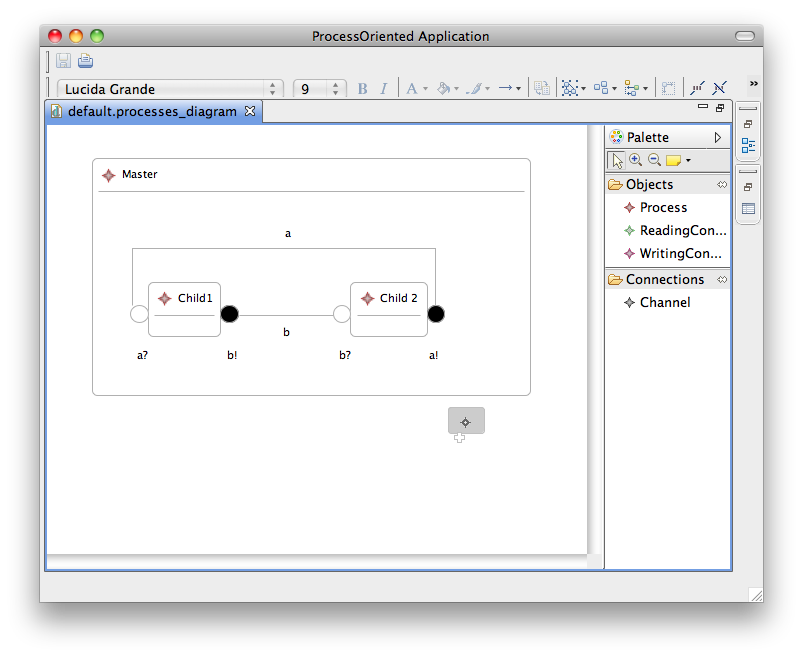
\includegraphics[scale=0.5]{A.2.ProcessOriented/images/6_model.png}
	\caption{Exemplar diagram after the final iteration.}
	\label{fig:po_it6_model}
\end{figure}

\section{Summary}
This appendix has described the way in which a graphical editor for process-oriented programs was designed and implemented using an iterative style of development. A metamodel was used to capture the key concepts of the domain, and to generate code for a graphical editor. Each iteration involved changing the metamodel either to correct unintended behaviour in the editor (iterations 3 and 5), to facilitate interoperability with other tools (iteration 2) or to add new features (iterations 1, 4 and 6). The metamodel changes described in the fifth iteration are used for evaluation of the thesis research in Section~\ref{sec:exemplar_user-driven_co-evo}.
